\title{Proyecto de Redes - Callcenter - PUJ, Cali.}
\author{Alejandro~Cardona,
        Luis~Santiago~Osorio}

\date{\today}

\documentclass[12pt]{article}
\hoffset - 1cm % 2cm
\voffset - 0.54cm % 2cm
\setlength{\textwidth}{15cm}
\baselinestretch
\renewcommand{\baselinestretch}{1.5}

\usepackage{dcolumn}
\usepackage{colortbl}
\usepackage{graphicx}
\usepackage{rotating}
\usepackage[utf8]{inputenc}
\usepackage[spanish]{babel}

\begin{document}
\maketitle
\pagebreak

\tableofcontents

\pagebreak 
\section{\textbf{Introduci\'on}}
En el desarrollo de una red para un callcenter, se aplicaran los pasos básicos de diseño, para obtener una solución que concuerde con los requerimientos necesarios de dicha red. En el proceso se realizaran los diseños y los cálculos de el consumo, espacio y demás, para hallar los elementos físicos necesarios y adecuados para el montaje de la red en donde no se haga desperdicio de recurso y se empleen los equipos y los elementos adecuados.\\\\

En este documento se mostrara el plano de la red, los equipos necesarios, tablas de comparación y demás, que respalden el buen diseño de la red y la buena selección de los equipos.

\pagebreak
\section{\textbf{Planteamiento del problema}}
Se necesita realizar el diseño de una red para un callcenter, equipado por 18 computadores que serán manejados por personal de la empresa, 2 computadores manejados en la oficina de dirección, servidores, y un servicio wifi, para la sala de visitas. En donde todos los computadores y dispositivos móviles, deberán poder tener acceso a internet, con sus debidas restricciones, en cuanto a el acceso a las diferentes redes internas del callcenter.\\\\
Además se debe garantizar una robustez en la red, ya que la conexión debe ser permanente para que no sea afectado el trabajo del callcenter.\\\\
Dentro de los problemas básicos que se abordaran serán los siguientes:
\begin{itemize}
\item
Proveedor de servicios
\item
Computadores
\item
infraestructura
\item
Robustez
\end{itemize}
\pagebreak
En el siguiente dibujo se muestra el plano del callcenter.
\begin{center}
\rotatebox{0}{\scalebox{1}[1]{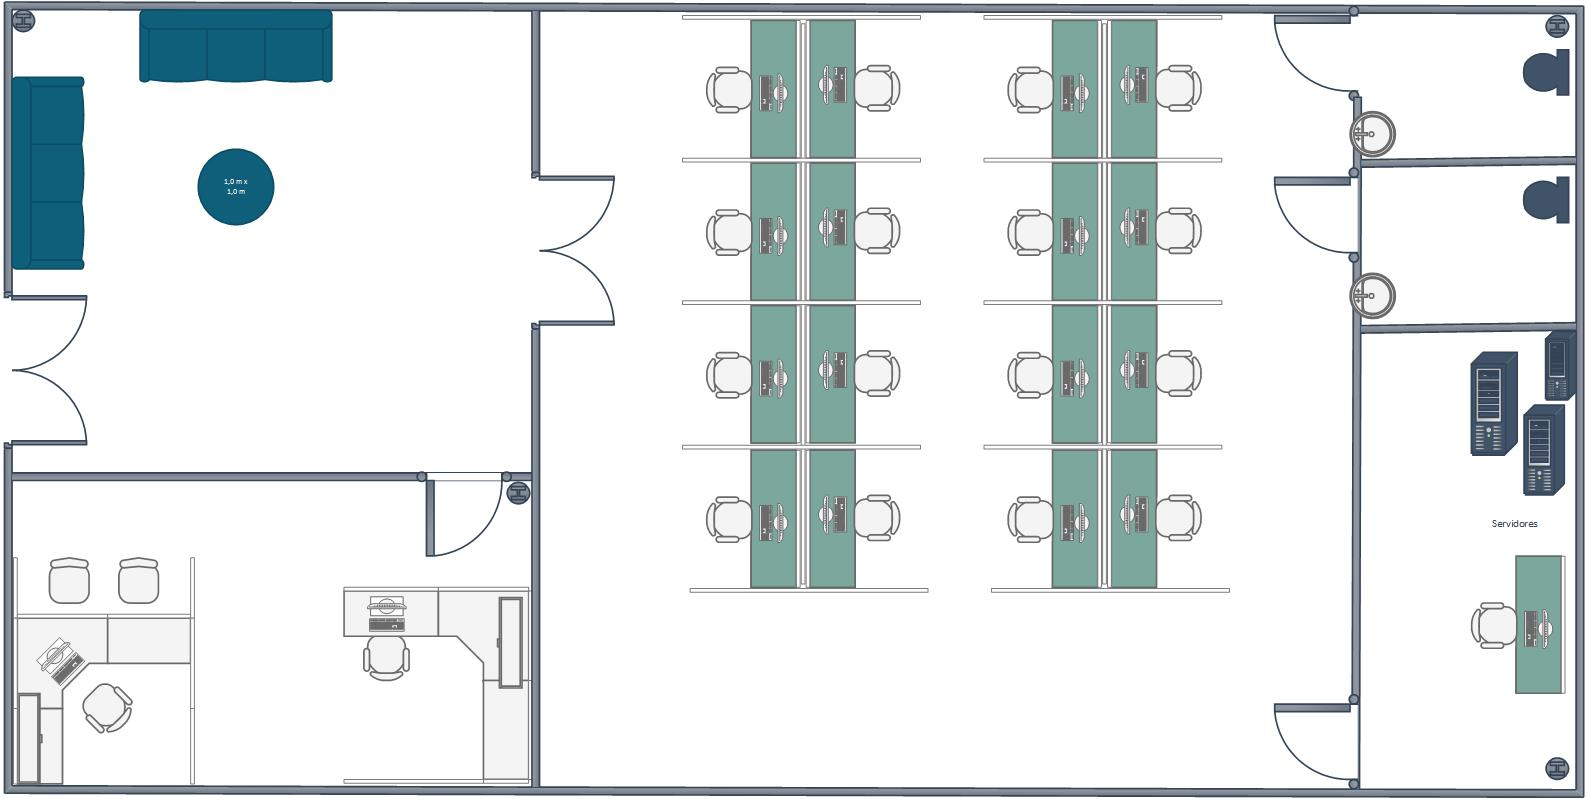
\includegraphics[width=16cm,height=9cm]{plano.jpg}}}
\end{center}
\pagebreak
\section{\textbf{Requerimienos de la red}}
Los requerimientos de la red para el callcenter serán los siguientes:
\begin{itemize}
\item
Numero de computadores.
\item
Conectividad Voip.
\item
Usuarios.
\item
Proveedor de internet.
\item
Tipos de cables.
\item
Velocidad.
\item
Costos.
\end{itemize}

\subsection{\textbf{Numero de computadores}}
En la red se tendrán al rededor de 30 a 42, con la siguiente distribución:
\begin{itemize}
\item
2-7 computadores en la oficina, 2 con punto de red y de 1 a 5 por acceso wifi.
\item
10 posibles accesos en la salada de espera, todos por acceso wifi.
\item
18 computadores en la sala de atención del callcenter, cada uno con su respectivo punto de red.
\item
5 puntos de acceso a cámaras de seguridad.
\end{itemize}

\subsection{\textbf{Conectividad VoIP}}
Debe existir conectividad Voip, tanto en los computadores de servicio como en los computadores de la oficina, ya que debido a que el software que se manejara para la atención del callcenter maneja la conectividad por VoIP.

%Analizar para terminar la tabla
\subsection{\textbf{Usuarios}}
Los usuarios de la red del callcenter, tendran la capacidad de desarrollar diferentes tareas y diferentes tipos de servicios en la red, los cuales se muestran acontinacion.\\\\
\begin{tabular}{|c|c|c|c|c|}
\hline
\makebox[3.1cm][c]{\textbf{Servicio/Usuario}} &\makebox[2.7cm][c]{\textbf{Pcs-Atencion}} &\makebox[2.7cm][c]{\textbf{Pcs-Oficina}} &\makebox[2.7cm][c]{\textbf{Pcs-Sala}} &\makebox[2.7cm][c]{\textbf{Seguridad}}\\
\hline
\makebox[2.7cm][c]{Nevegacion Web} &\makebox[2.7cm][c]{No} &\makebox[2.7cm][c]{Si} &\makebox[2.7cm][c]{Si} &\makebox[2.7cm][c]{No}\\
\hline
\makebox[2.7cm][c]{VoIp} &\makebox[2.7cm][c]{Si} &\makebox[2.7cm][c]{Si} &\makebox[2.7cm][c]{No} &\makebox[2.7cm][c]{No}\\
\hline
\makebox[2.7cm][c]{Descargas} &\makebox[2.7cm][c]{No} &\makebox[2.7cm][c]{Si} &\makebox[2.7cm][c]{Si} &\makebox[2.7cm][c]{No}\\
\hline
\makebox[2.7cm][c]{Video llamadas} &\makebox[2.7cm][c]{Si} &\makebox[2.7cm][c]{Si} &\makebox[2.7cm][c]{No} &\makebox[2.7cm][c]{No}\\
\hline
\makebox[2.7cm][c]{OS} &\makebox[2.7cm][c]{Windows} &\makebox[2.7cm][c]{Windows} &\makebox[2.7cm][c]{All} &\makebox[2.7cm][c]{Otro}\\
\hline
\end{tabular}

\subsection{\textbf{Proveedor de internet}}
Se requiere que se tengan 2 proveedores de internet para que exista una robustez en la red, ya que debido a que es un callcenter, la conexión deberá ser continua y sin interrupciones, también se debe tener en cuenta la calidad del servicio del proveedor en cuanto a una respuesta a fallos en la red y si el servicio cumple con las necesidades de los usuarios.

\subsection{\textbf{Cables}}
Los tipos de cables para la red, deben soportar el trafico de red y garantizar conexión.

\subsection{\textbf{Velocidad}}
La velocidad de conexión debe ser efectiva y continua, para poder sostener las llamadas del callcenter, y que siempre exista una comunicación fluida con los clientes del callcenter.

\subsection{\textbf{Costo}}
El costo de la red es libre, se cuenta con el capital para cualquier inversión, siempre y cuando esta inversión este justificada.

\pagebreak
\section{\textbf{Distrucibucion de el paso de los cables}}
En esta sección del documento se muestra un plano de la distribución, a los diferentes equipos finales de la red, como lo son los computadores de la oficina de la sala del callcenter y el accespoint para la sala.

\begin{center}
\rotatebox{0}{\scalebox{1}[1]{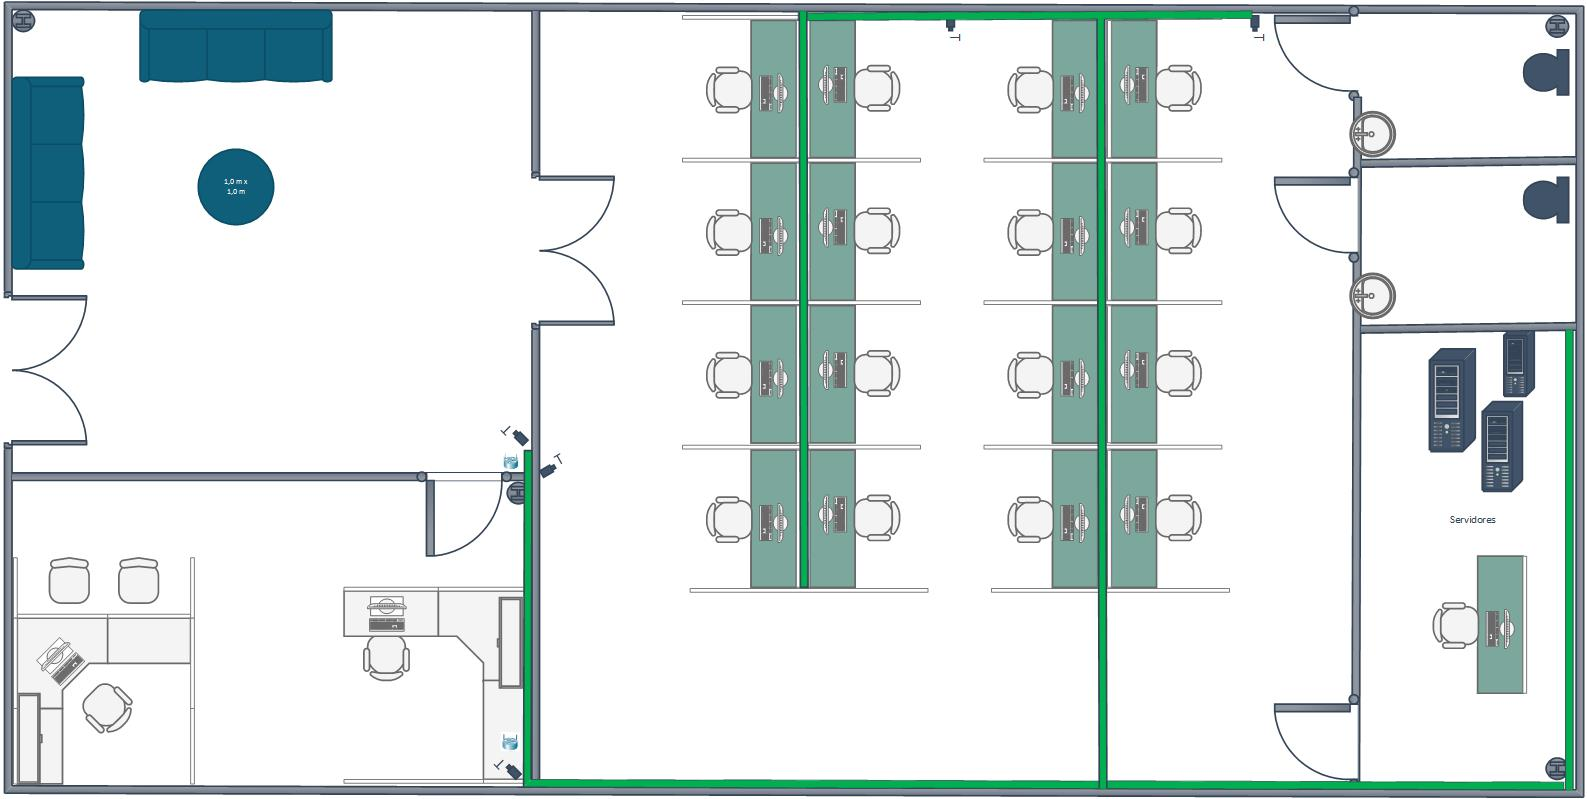
\includegraphics[width=16cm,height=9cm]{planocanaletas.jpg}}}
\end{center}


\pagebreak
\section{\textbf{Analisis de consumo}}
Dentro de los requerimientos de la red, se tendrán en cuenta para el análisis del trafico aquellos en los que aya un mayor uso por parte de los usuarios del callcenter, para poder posteriormente, hacer las posibles evaluaciones de selección del proveedor de servicio, selección de los equipos a utilizar y de los diferentes materiales de infraestructura que se utilizaran.\\\\
En los servicios que se deben prestar para el callcenter los mas utilizados son el manejo de VoIP y las cámaras de seguridad debido a que tienen un flujo continuo sobre la red, y la navegación web para los computadores que no están restringidos.\\\\
%% Para el analizis del consumo se tendran en cuenta los diferentes tipos de servicio que se le ofreceran a los usuarios de la red.\\\\
%% Los servicios son los siguentes:
%% \begin{itemize}
%% \item
%% Navegacion Web.
%% \item
%% VoIP.
%% \item
%% Descargas.
%% \item
%% Video llamadas.
%% \item
%% Camaras de seguridad.
%% \end{itemize}

\subsection{\textbf{Consumo VoIP}}
En el consumo VoIP, se tiene en cuenta que este servicio consta de 2 etapas, la señalización de la llamada y la transmisión de audio que es realizada a través de RTP, dado a que el ancho de banda consumido por la señalización no es relevante, se enfocara el calculo de consumo en la transmisión del audio.\\\\
Para el análisis de esta transmisión veremos el empaquetamiento de los datos en las 7 capas del modelo OSI. El audio codificado necesita ser empaquetado dentro de paquetes RTP. A su vez, los paquetes RTP necesitan ser empaquetados dentro de paquetes UDP, que luego necesitan ser empaquetados dentro de paquetes IP. en este ejemplo tomaremos Ethernet que es el tipo de red más común, y requiere otro empaquetamiento.\\\\
En la siguiente tabla se ilustra lo dicho, con los respectivos valores para cada una de las capaz.\\\\

\begin{tabular}{|c|c|}
\hline
\makebox[3.1cm][c]{Ethernet} &\makebox[3.1cm][c]{15.2 kbps}\\
\hline
\makebox[2.7cm][c]{IP} &\makebox[3.1cm][c]{8 kbps}\\
\hline
\makebox[2.7cm][c]{UDP} &\makebox[3.1cm][c]{3.2 kbps}\\
\hline
\makebox[2.7cm][c]{RTP} &\makebox[3.1cm][c]{4.8 kbps}\\
\hline
\makebox[2.7cm][c]{Encoded Audio} &\makebox[3.1cm][c]{Depende del codec}\\
\hline
\end{tabular}\\\\\\
Los codecs de audio para el VoIP, son el G711, G722, GSM Y G729 en los cuales veremos diferentes características y tomaremos el mas indicado para el callcenter.\\\\

\begin{tabular}{|c|c|c|c|}
\hline
\makebox[3.1cm][c]{\textbf{Codec}} &\makebox[3.1cm][c]{\textbf{Calidad Audio}} &\makebox[3.1cm][c]{\textbf{Recursos CPU}} &\makebox[3.1cm][c]{\textbf{Tamaño}}\\
\hline
\makebox[2.7cm][c]{G711} &\makebox[3.1cm][c]{Buena} &\makebox[3.1cm][c]{Muy pocos} &\makebox[3.1cm][c]{95.2}\\
\hline
\makebox[2.7cm][c]{G722} &\makebox[3.1cm][c]{Muy Buena} &\makebox[3.1cm][c]{Pocos} &\makebox[3.1cm][c]{95.2}\\
\hline
\makebox[2.7cm][c]{GSM} &\makebox[3.1cm][c]{Aceptable} &\makebox[3.1cm][c]{Promedio} &\makebox[3.1cm][c]{44.2}\\
\hline
\makebox[2.7cm][c]{G729} &\makebox[3.1cm][c]{Promedio} &\makebox[3.1cm][c]{Altos} &\makebox[3.1cm][c]{39.2}\\
\hline
\end{tabular}\\\\
Según las tablas anteriormente mostradas, el codec adecuado para el callcenter será el G722, ya que uno de los principales requerimientos es que debe haber una buena comunicación, se utilizara este codec y debido a que se cuenta con los recursos necesarios se adaptara la red para tener el uso de este codec.\\\\
En un total el consumo de uno de los equipos para el uso de este servicio seria el siguiente en cuanto a kbps:\\\\

\begin{tabular}{|c|c|}
\hline
\makebox[3.1cm][c]{Ethernet} &\makebox[3.1cm][c]{15.2 kbps}\\
\hline
\makebox[2.7cm][c]{IP} &\makebox[3.1cm][c]{8 kbps}\\
\hline
\makebox[2.7cm][c]{UDP} &\makebox[3.1cm][c]{3.2 kbps}\\
\hline
\makebox[2.7cm][c]{RTP} &\makebox[3.1cm][c]{4.8 kbps}\\
\hline
\makebox[2.7cm][c]{Encoded Audio} &\makebox[3.1cm][c]{64 kbps}\\
\hline
\makebox[2.7cm][c]{\textbf{Total}} &\makebox[3.1cm][c]{\textbf{95.2 kbps}}\\
\hline
\end{tabular}\\\\\\
De acuerdo con los cálculos, cada equipo de los usuarios de atención y de los usuarios de oficina consumirá un total de 95.2 kbps, y teniendo en cuenta la calidad media de conexión de equipos en la red el consumo por kbps seria de 18 * 95.2 kbps dándonos un total medio de consumo de VoIP de 1713.6 kbps.

\subsection{\textbf{Consumo TCP/IP Cámaras de seguridad}}
El sistema de vigilancia del callcenter Serra de tipo IP, el cual utilizara los recursos TCP/IP de la red para enviar video y audio de cada cámara a el servidor dedicado del sistema de vigilancia. el calculo de ancho de banda para las cámaras de seguridad esta dado, según la resolución que envíen las cámaras al servidor. El sistema de seguridad del callcenter se realizara en formato de video MPEG4. En la siguiente tabla se muestra algunas de las resoluciones y sus valores de consumo de banda ancha para el formato MPEG4.\\\\
\begin{tabular}{|c|c|c|}
\hline
\makebox[3.1cm][c]{\textbf{Resolucion}} &\makebox[3.1cm][c]{\textbf{IPS}} &\makebox[3.1cm][c]{\textbf{Kbps}}\\
\hline
\makebox[3.1cm][c]{CIF} &\makebox[3.1cm][c]{3} &\makebox[3.1cm][c]{160}\\
\hline
\makebox[3.1cm][c]{CIF} &\makebox[3.1cm][c]{7} &\makebox[3.1cm][c]{185}\\
\hline
\makebox[3.1cm][c]{CIF} &\makebox[3.1cm][c]{15} &\makebox[3.1cm][c]{200}\\
\hline
\makebox[3.1cm][c]{CIF} &\makebox[3.1cm][c]{30} &\makebox[3.1cm][c]{500}\\
\hline
\makebox[3.1cm][c]{2CIF} &\makebox[3.1cm][c]{3} &\makebox[3.1cm][c]{320}\\
\hline
\makebox[3.1cm][c]{2CIF} &\makebox[3.1cm][c]{7} &\makebox[3.1cm][c]{370}\\
\hline
\makebox[3.1cm][c]{2CIF} &\makebox[3.1cm][c]{15} &\makebox[3.1cm][c]{400}\\
\hline
\makebox[3.1cm][c]{2CIF} &\makebox[3.1cm][c]{30} &\makebox[3.1cm][c]{1000}\\
\hline
\makebox[3.1cm][c]{4CIF} &\makebox[3.1cm][c]{3} &\makebox[3.1cm][c]{640}\\
\hline
\makebox[3.1cm][c]{4CIF} &\makebox[3.1cm][c]{7} &\makebox[3.1cm][c]{740}\\
\hline
\makebox[3.1cm][c]{4CIF} &\makebox[3.1cm][c]{15} &\makebox[3.1cm][c]{800}\\
\hline
\makebox[3.1cm][c]{4CIF} &\makebox[3.1cm][c]{30} &\makebox[3.1cm][c]{2000}\\
\hline
\end{tabular}\\\\\\

La calidad requerida para el callcenter será 2CIF a 15 IPS, que es el formato mas común y de buena calidad para la imagen. Dados los datos el consumo de las cámaras de seguridad en la red común de 400 kbps por cada cámara, dándonos un tota de 5 * 400 la suma de el trafico de todas las cámaras de seguridad, para un total de 2000 kbps.

\subsection{\textbf{Consumo Navegación web, chat, videos, email}}
El calculo de el trafico consumido por la navegación web, chat, videos y email se realizara con un simulador Capsa de Colasoft, en el cual se realizo una medición de un solo ordenador efectuando las tareas descritas. El resultado fue que el computador realizando estas tareas tiene un consumo de alrededor de 36 kbps, lo cual nos dará un total de consumo para los computadores que no tienen esta restricción de 17 * 36 kbps tomando el peor de los casos en los que estén todos los pcs conectados sin restricción para un total de 612 kbps.

\subsection{\textbf{Consumo Total}}
El consumo total en la red se mostrara en el siguiente plano del callcenter, en el que se observaran los distintos tipos de consumos sacados anteriormente, ya que son los mas importantes en la red.\\\\
\subsubsection{\textbf{Plano de consumo}}
\begin{center}
\rotatebox{0}{\scalebox{1}[1]{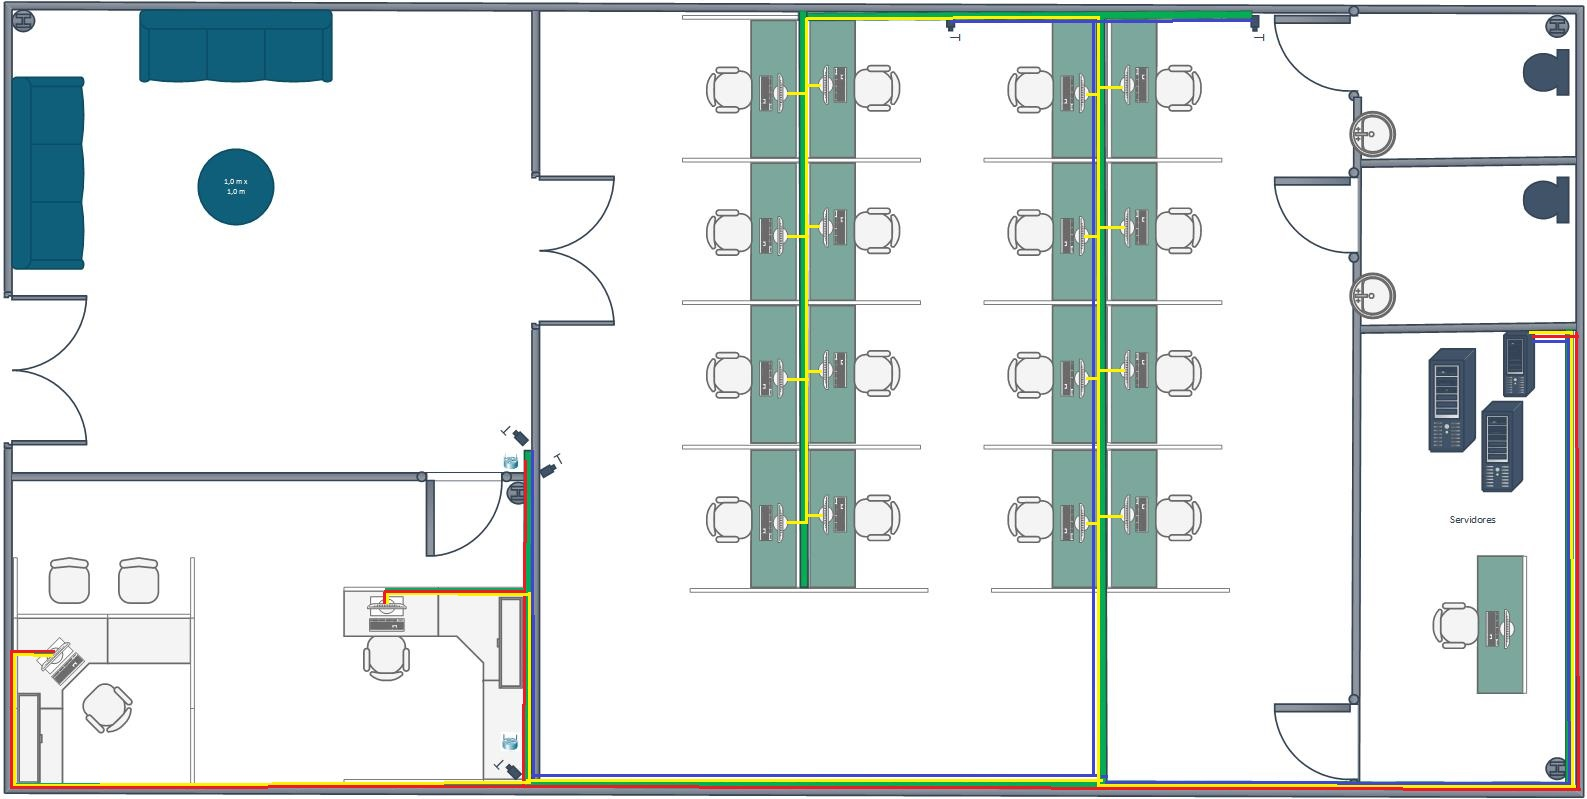
\includegraphics[width=16cm,height=9cm]{planoconsumo.jpg}}}
\end{center}
\subsubsection{\textbf{Consumo por servicio}}
En el plano se observa el flujo de consumo de cada uno de los servicios fundamentales de la red. en la siguiente tabla se explica cada color y si el servicio consume de subida y de bajada.\\\\
\begin{tabular}{|c|c|c|c|}
\hline
\makebox[3.1cm][c]{\textbf{Color}} &\makebox[3.1cm][c]{\textbf{Servicio}} &\makebox[3.1cm][c]{\textbf{Download}} &\makebox[3.1cm][c]{\textbf{Upload}}\\
\hline
\makebox[3.1cm][c]{Amarillo} &\makebox[3.1cm][c]{VoIP} &\makebox[3.1cm][c]{Si} &\makebox[3.1cm][c]{Si}\\
\hline
\makebox[3.1cm][c]{Rojo} &\makebox[3.1cm][c]{NavegacionWeb} &\makebox[3.1cm][c]{si} &\makebox[3.1cm][c]{Poco}\\
\makebox[3.1cm][c]{} &\makebox[3.1cm][c]{y otros} &\makebox[3.1cm][c]{} &\makebox[3.1cm][c]{}\\
\hline
\makebox[3.1cm][c]{Azul} &\makebox[3.1cm][c]{Seguridad} &\makebox[3.1cm][c]{Poco} &\makebox[3.1cm][c]{Si}\\
\hline
\end{tabular}\\\\

\begin{itemize}
\item
\textbf{VoIP(Amarillo)}: El consumo de VoIP en el cable amarillo, segun el consumo calculado es de 95.2 por equipo, y segun la tabla anterior, este consumo estara de subida y bajada por lo que el trafico en el cable amarillo por computador con acceso a este servicio sera un total de 190.4 kbps.
\item
\textbf{NavegacionWeb y otros(Rojo)}: El consumo de este servicio es un consumo que tiene su gran parte de trafico en la descarga por lo que no tendremos en cuenta el poco trafico de subida. Para cada uno de los equipos con este servicio el consumo de navegacion sera entonces 36 Kbps.
\item
\textbf{Seguridad(Azul)}: El consumo de la seguridad, muestra que es poco su consumo de descarga ya que este servicio tiene un mayor de consumo de subida, por el envio de las imagenes y audio, caculados previamente, en este servicio tendremos en cuenta su consumo de subida, el cual nos dara un total de 400 Kbps por camara. 
\end{itemize}
El total consumido en los sectores del callcenter, se muestra en el plano de consumo y estara definido por la cantidad de colores que pasen por la canaleta y los computadores ligados en ese momento a dicho color.\\\\ 

\pagebreak
\section{\textbf{Equipos}}
Los equipos que utilizaremos para el callcenter, estarán seleccionados según los cálculos de consumo hechos anteriormente y se mostraran las especificaciones necesarias para la red de cada equipo, que nos permita tomar una decisión acerca de cual es mejor para nuestra red.\\\\
En la red observamos que tenemos un consumo de descarga en su punto máximo de 5372 Kbps y de subida de 6760 kbps.En la siguiente tabla se muestra los calculos de subida y de bajada.
\begin{itemize}
\item
\textbf{Calculo de bajada}:\\\\
\begin{tabular}{|c|c|c|c|}
\hline
\makebox[3.1cm][c]{\textbf{Servicio}} &\makebox[3.1cm][c]{\textbf{Consumo}} &\makebox[3.1cm][c]{\textbf{NoEquipos}} &\makebox[3.1cm][c]{\textbf{Total}}\\
\hline
\makebox[3.1cm][c]{VoIP} &\makebox[3.1cm][c]{190.4 Kbps} &\makebox[3.1cm][c]{25} &\makebox[3.1cm][c]{4760 Kbps}\\
\hline
\makebox[3.1cm][c]{NavegacionWeb} &\makebox[3.1cm][c]{36 Kbps} &\makebox[3.1cm][c]{17} &\makebox[3.1cm][c]{612 Kbps}\\
\makebox[3.1cm][c]{y otros} &\makebox[3.1cm][c]{} &\makebox[3.1cm][c]{} &\makebox[3.1cm][c]{}\\
\hline
\makebox[3.1cm][c]{} &\makebox[3.1cm][c]{} &\makebox[3.1cm][c]{\textbf{Total}} &\makebox[3.1cm][c]{5370 Kbps}\\
\hline
\end{tabular}
\item
\textbf{Calculo de subida}:\\\\
\begin{tabular}{|c|c|c|c|}
\hline
\makebox[3.1cm][c]{\textbf{Servicio}} &\makebox[3.1cm][c]{\textbf{Consumo}} &\makebox[3.1cm][c]{\textbf{NoEquipos}} &\makebox[3.1cm][c]{\textbf{Total}}\\
\hline
\makebox[3.1cm][c]{VoIP} &\makebox[3.1cm][c]{190.4 Kbps} &\makebox[3.1cm][c]{25} &\makebox[3.1cm][c]{4760 Kbps}\\
\hline
\makebox[3.1cm][c]{Seguridad} &\makebox[3.1cm][c]{400 Kbps} &\makebox[3.1cm][c]{5} &\makebox[3.1cm][c]{2000 Kbps}\\
\hline
\makebox[3.1cm][c]{} &\makebox[3.1cm][c]{} &\makebox[3.1cm][c]{\textbf{Total}} &\makebox[3.1cm][c]{6760 Kbps}\\
\hline
\end{tabular}
\end{itemize} 

\pagebreak
\subsection{\textbf{Equipos de la red}}
En la siguente lista se mostraran los equipos que se utilizaran en la red.
\begin{itemize}
\item
4 Routers.
\item
4 Switches.
\item
2 Acces Point.
\item
Computadores.
\item
Servidor Camaras de seguridad.
\item
Servidor VoIP. 
\end{itemize}

\subsection{\textbf{Routers}}
En esta sección del documento se mostraran algunas comparaciones, características de los routers para realizar la selección de los routers indicados para la red.\\\\
\begin{tabular}{|c|c|c|c|c|}
\hline
\makebox[2.5cm][c]{\textbf{Marca}} &\makebox[2.5cm][c]{\textbf{Router}} &\makebox[2.5cm][c]{\textbf{Puertos}} &\makebox[2.5cm][c]{\textbf{Mbps}} &\makebox[2.5cm][c]{\textbf{Frecuencia}}\\
\makebox[2.5cm][c]{} &\makebox[2.5cm][c]{} &\makebox[2.5cm][c]{\textbf{FastEthernet}} &\makebox[2.5cm][c]{} &\makebox[2.5cm][c]{}\\
\hline
\makebox[2.5cm][c]{D-link} &\makebox[2.5cm][c]{AC1000} &\makebox[2.5cm][c]{4} &\makebox[2.5cm][c]{300} &\makebox[2.5cm][c]{2.4GHz}\\
\hline
\makebox[2.5cm][c]{Huawei} &\makebox[2.5cm][c]{E5776} &\makebox[2.5cm][c]{4} &\makebox[2.5cm][c]{150} &\makebox[2.5cm][c]{2.4GHz}\\
\hline
\makebox[2.5cm][c]{Cisco} &\makebox[2.5cm][c]{1812/K9} &\makebox[2.5cm][c]{8} &\makebox[2.5cm][c]{100} &\makebox[2.5cm][c]{2.4GHz}\\
\hline
\end{tabular}\\\\
En la selección del router se escoge el router Cisco debido que a pesar de que el costo es un poco mas elevado, posee la velocidad necesaria y adecuada para el callcenter y tiene un mejor soporte que los otros 2 routers.\\\\

\subsection{\textbf{Switches}}
En esta sección del documento se mostraran algunas comparaciones, características de los switches para realizar la selección de los switches indicados para la red.\\\\
\begin{tabular}{|c|c|c|c|}
\hline
\makebox[2.5cm][c]{\textbf{Marca}} &\makebox[2.5cm][c]{\textbf{Switche}} &\makebox[2.5cm][c]{\textbf{Puertos}} &\makebox[2.5cm][c]{\textbf{RackMountable}}\\
\hline
\makebox[2.5cm][c]{Cisco} &\makebox[3.2cm][c]{WS-C2960-24TT-L} &\makebox[2.5cm][c]{24} &\makebox[3cm][c]{Si}\\
\hline
\makebox[2.5cm][c]{Cisco} &\makebox[2.5cm][c]{WS-C3560X-24T-L} &\makebox[2.5cm][c]{24} &\makebox[2.5cm][c]{Si}\\
\hline
\makebox[2.5cm][c]{D-link} &\makebox[2.5cm][c]{DES-108} &\makebox[2.5cm][c]{8} &\makebox[2.5cm][c]{No}\\
\hline
\makebox[2.5cm][c]{D-link} &\makebox[2.5cm][c]{DGS-1024A} &\makebox[2.5cm][c]{24} &\makebox[2.5cm][c]{No}\\
\hline
\makebox[2.5cm][c]{D-link} &\makebox[2.5cm][c]{DSS-16+} &\makebox[2.5cm][c]{16} &\makebox[2.5cm][c]{Si}\\
\hline
\end{tabular}\\\\
En la selección del switche, se toma el switche cisco WS-C2960-24TT-L, ya que a pesar de que los dos switches cumplen con las características principales de la red, no es necesario del switche WS-C3560X-24T-L, que tenga tantas opciones de conexión remota ya que la red se manejara internamente en el callcenter, para el manejo de la red de los pcs de la oficina ya que el router tiene un switche integrado, no abra neecidad de switche, ya que la capacidad requerida no supera los puertos de conexion del router.

\subsection{\textbf{Acces point}}
En esta sesión del documento se mostraran algunas comparaciones, características de los accespoint para realizar la selección de los accespoint indicados para la red.\\\\

\begin{tabular}{|c|c|c|}
\hline
\makebox[2.5cm][c]{\textbf{Marca}} &\makebox[2.5cm][c]{\textbf{Acccespoint}} &\makebox[2.5cm][c]{\textbf{band}}\\
\hline
\makebox[2.5cm][c]{Cisco} &\makebox[3.2cm][c]{AIR-AP1261N-A-K9} &\makebox[2.5cm][c]{5GHz}\\
\hline
\makebox[2.5cm][c]{D-link} &\makebox[3.2cm][c]{DAP-1522} &\makebox[2.5cm][c]{2.4GHz}\\
\hline
\end{tabular}\\\\
Se selecciona el accespoint de cisco AIR-AP1261N-A-K9, ya que tiene una mejor frecuencia.\\\\

\pagebreak
\section{\textbf{Mapa de coexiones de la red y Rack}}
A continuación se mostrara el mapa de la red física y la relación entre cada dispositivo.

\begin{center}
\rotatebox{0}{\scalebox{1}[1]{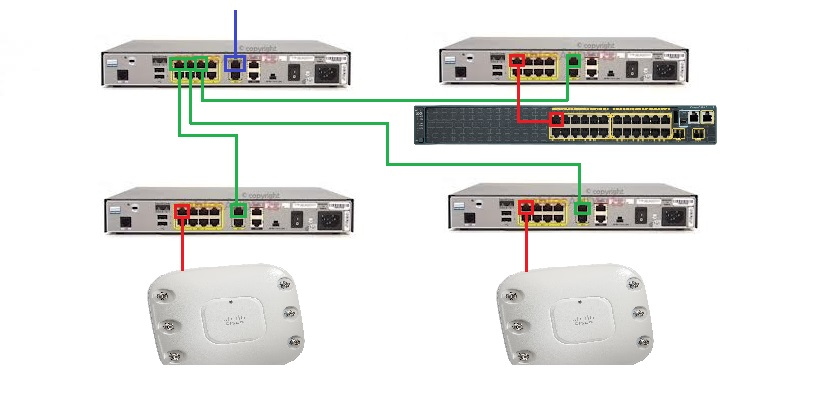
\includegraphics[width=10cm,height=8cm]{conred.jpg}}}
\end{center}
En la imagen se observa las conexiones entre los router switches y accespoint de la red. En la señalización, el color azul, representa la entrada de los dos proveedores de Internet. El color verde las conexiones entre los routers internos para las subredes y el color rojo, la conexión de salida de los routers internos a los dispositivos necesarios.\\\\
\pagebreak

En la siguiente imagen se mostrara la organización del rack con los dispositivos que se encuentren en el, ya que los accespoint no estarán presentes en el rack.\\\\
\begin{center}
\rotatebox{0}{\scalebox{1}[1]{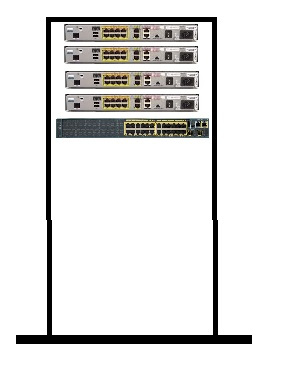
\includegraphics[width=10cm,height=8cm]{rack.jpg}}}
\end{center}

\pagebreak
\section{\textbf{VLCM de la red}}
para el manejo de las direcciones de red, se manejo protocolo de enrrutamiento RIP v2 y VLCM para la asignación de las IP, en la siguiente tabla se muestra la asignación de cada IP a las redes internas necesarias dentro del callcenter.

\begin{itemize}
\item
Red central = A.
\item
Red Oficina = B.
\item
Red de Sala de Atencion callcenter = C.
\item
Red Sala de visitas = D.
\end{itemize}

\begin{tabular}{|c|c|c|c|c|}
\hline
\makebox[2.5cm][c]{\textbf{Red}} &\makebox[2.5cm][c]{\textbf{Pcs}} &\makebox[2.5cm][c]{\textbf{Direccion}} &\makebox[2.5cm][c]{\textbf{Mask}} &\makebox[2.5cm][c]{\textbf{Rango}}\\
\hline
\makebox[2.5cm][c]{C} &\makebox[3.2cm][c]{18} &\makebox[2.5cm][c]{192.168.0.0} &\makebox[2.5cm][c]{255.255.255.224} &\makebox[2.5cm][c]{.1 - .30}\\
\hline
\makebox[2.5cm][c]{D} &\makebox[3.2cm][c]{10} &\makebox[2.5cm][c]{192.168.0.32} &\makebox[2.5cm][c]{255.255.255.240} &\makebox[2.5cm][c]{.33 - .46}\\
\hline
\makebox[2.5cm][c]{B} &\makebox[3.2cm][c]{7} &\makebox[2.5cm][c]{192.168.0.48} &\makebox[2.5cm][c]{255.255.255.240} &\makebox[2.5cm][c]{.49 - .62}\\
\hline
\makebox[2.5cm][c]{A} &\makebox[3.2cm][c]{4} &\makebox[2.5cm][c]{192.168.0.64} &\makebox[2.5cm][c]{255.255.255.248} &\makebox[2.5cm][c]{.65 - .70}\\
\hline
\end{tabular}\\\\


\pagebreak
\section{\textbf{Simulacion Packet Tracer}}
El diseño de la red se simulo en el Cisco Packet Tracer, en donde se genero el plano de la red con las especificaciones requeridas y se demostró conexión entre los equipos y a la salida de internet.

\subsection{\textbf{Plano Packet Tracer}}
\begin{center}
\rotatebox{0}{\scalebox{1}[1]{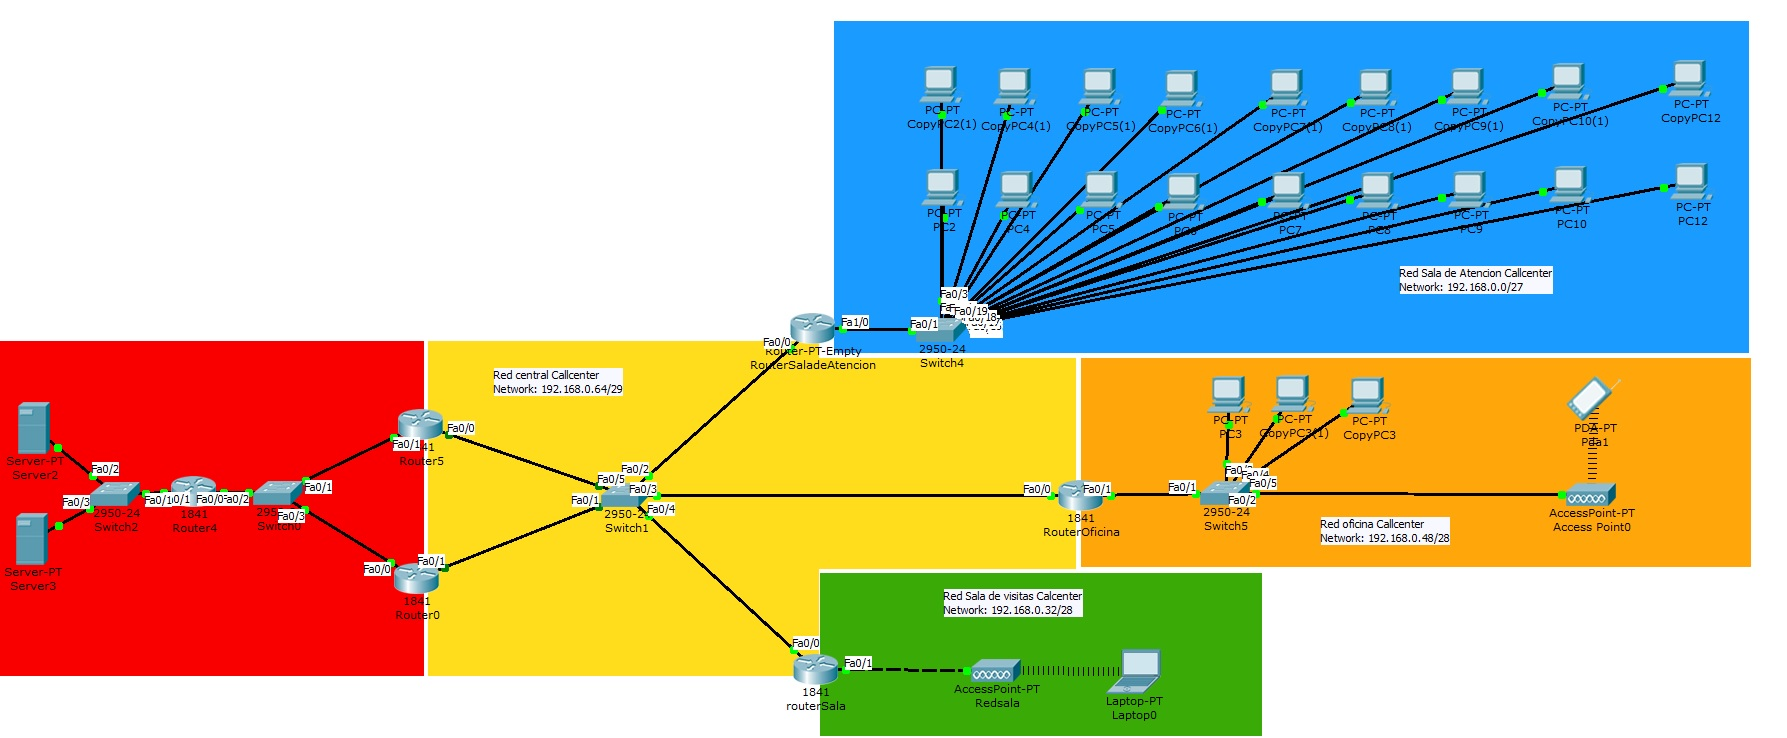
\includegraphics[width=17cm,height=12cm]{planopkt.jpg}}}
\end{center}


\bibliographystyle{abbrv}
\bibliography{main}

\end{document}

